\documentclass[pdftex,12pt,a4paper]{article}


\usepackage[pdftex]{graphicx}
\usepackage[utf8]{inputenc}
\usepackage{import}
\usepackage{listings}
\usepackage{color}
\usepackage{hyperref}
\usepackage{titlesec}
\usepackage{subcaption}
\usepackage{placeins}
\usepackage{capt-of}
\usepackage[font=scriptsize]{caption}
\usepackage{tocloft}
\usepackage[utf8]{inputenc}
\usepackage[english]{babel}
\usepackage{amsmath}
\usepackage{biblatex}

\pagenumbering{arabic}



\addbibresource{biblo.bib}
\hypersetup{%
    pdfborder = {0 0 0}
}


%\titleformat{\section}[block]{\Large\bfseries\filcenter}{}{1em}{}
%\titleformat{\paragraph}[block]{\bfseries\filcenter}{}{1em}{}

\setlength{\parindent}{0em}
\setlength{\parskip}{1em}

\newcommand\myworries[1]{\textcolor{red}{#1}}
\newcommand{\HRule}{\rule{\linewidth}{0.5mm}}
\newcommand{\inlinecode}{\texttt}
\newcommand*{\blankpage}{%
  \vspace*{\fill}
  \begin{center}
      This page is left intentionally blank.
  \end{center}
  \vspace{\fill}%

  \clearpage
}

 


\begin{document}

    % Table of content line spacing
    \setlength\cftparskip{0pt}
    \setlength\cftbeforesecskip{10pt}
    \setlength\cftbeforesubsecskip{2pt}
    \setlength\cftaftertoctitleskip{22pt}

    % Title Page (0)
    % http://en.wikibooks.org/wiki/LaTeX/Title_Creation


\begin{titlepage}
\begin{center}

% Upper part of the page. The '~' is needed because \\
% only works if a paragraph has started.

\includegraphics[width=0.7\textwidth]{./uia_eng}~\\[2cm]


\textsc{\Large IKT-416 Short project expose}\\[0.5cm]

% Title
\HRule \\[0.4cm]
{ \huge \bfseries T-FLIP Adaptive Learning \\[0.4cm] }

\HRule \\[1.5cm]

% Author and supervisor
\noindent
\begin{minipage}[t]{0.4\textwidth}
\begin{flushleft} \large
\emph{Authors:}\\
Per-Arne \textsc{Andersen}
Christian \textsc{Kråkevik}
\end{flushleft}
\end{minipage}%
\begin{minipage}[t]{0.4\textwidth}
\begin{flushright} \large
\emph{Supervisors:} \\

Martin Wulf \textsc{Gerdes}\\
\end{flushright}
\end{minipage}

\vfill

% Bottom of the page
{\large \today}

\end{center}
\end{titlepage}
    \clearpage
    
    % Blank Page (1)
    \blankpage

    % Table of contents (3)
    \tableofcontents

    \clearpage


        
      % Content Page (0)
    
\section{Introduction}
The goal is to research and implement an algorithm to distribute relevant programming tasks to students. This algorithm will classify each individual student based on skill level. 

Such algorithm is generally referred to as a "Student Model" or  Computerized adaptive testing (CAT)\cite{CAT}. The model aims to place a student in a given group based on experience. The selection is made with initial tasks that aims to place the student in a correct group correlating with the student's skill-level. 

The created algorithm should be able to identify this skill-set. As the student answers more questions the algorithm should fine-tune the skill variable to match the student skill as close as possible. 

The project aims to provide the student with course content that matches their own learning style, this will hopefully make the students learning rate quicker and more efficient.

\clearpage


\section{About}
"Testdrevet ferdighetslærling i programmering" (T-FLIP) \cite{website:tflip} is a university project funded by the University of Agder and Norgesuniversitetet. The main purpose of this project is to create a framework for automated testing of student tasks.
The project is due in 2017

\subsection{Why}
This project is a test, to see if adaptive learning can be combined with the pre-existing T-FLIP framework, thus giving the product the ability to both check and give tasks. 



\subsection{Research questions}

The project aims to research if the bandit-algorithm or a descendant of this algorithm can be used to improve the learning rate / efficiency of students in a programming class.


\clearpage

\section{State of art}
There is a lot of research done in the field of adaptive learning, and there are already systems in place for classroom environments.

An example of such software is "dreambox"
\begin{figure}[!htb]
    \centering
    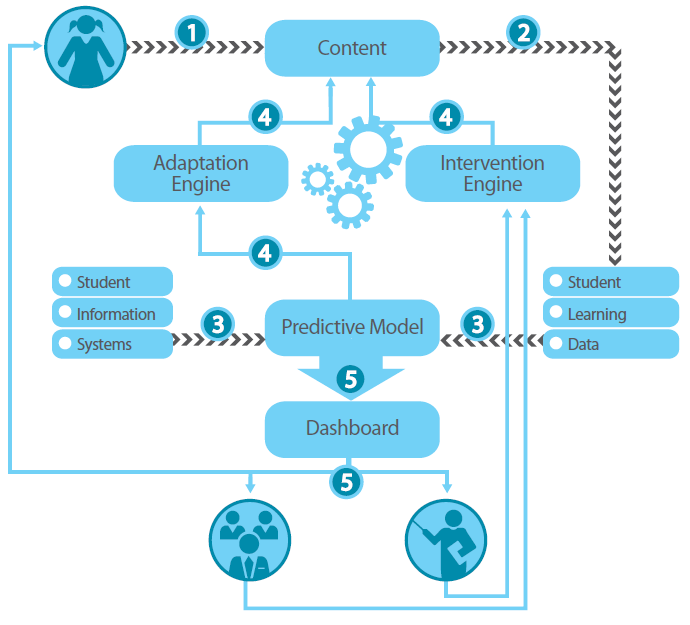
\includegraphics[width=0.8\textwidth]{./adaptive.png}
    \caption{Dreambox adaptive learning model}
    \label{fig:awesome_image}
\end{figure}

More can be read about their model in their published white paper\cite{website:dreambox}.

The main goal of our project is to research how these companies resolve this problem, and develop an algorithm suited for adaptive learning in programming topics. 

Several approaches is documented as peer-reviewed studies both using bandit-algorithms and bayanes-networks.\cite{baynet}\cite{mabits}


\section{Purposed solution}

\subsection {Algorithms, Which Approach?}

Alot of research has been done in order to find a algorithm well suited for this task. Starting this project, the main focus will be Bandit algorithms, Learning automata's and a proposed algorithm called Hobbit-Hood.

Attempts to implement a useable multi-armed bandit (MAB) will be attempted in this project. MAB may be suited as its purpose is to find an optimal choice from a number of possible selection, which is an requirement of the task.
It is however uncertain that MAB will work as it is usually used as a "single optimal finder".

To counter this, an alternative algorithm made by the project participants may be used. This algorithm is called "Hobbit Hood", which are in many cases works like a Bandit. The difference between these algorithms is that Hobbit Hood makes it possible for finding multiple optimals instead of just one. It is still not certain whether it has the capacity to find the optimal.

    \begin{figure}[!htb]
        \begin{bmatrix}
        0.8 & 0 & 0 & 0 & 0 & 0 & 0 & 0 & 0 & 0 \\
        0.1 & 0 & 0 & 0 & 0 & 0 & 0 & 0 & 0 & 0 \\
        0.0 & 0 & 0 & 0 & 0 & 0 & 0 & 0 & 0 & 0 \\
        0.0 & 0 & 0 & 0 & 0 & 0 & 0 & 0 & 0 & 0 \\
        0.0 & 0 & 0 & 0 & 0 & 0 & 0 & 0 & 0 & 0 \\
        0.0 & 0 & 0 & 0 & 0 & 0 & 0 & 0 & 0 & 0 \\
        0.1 & 0 & 0 & 0 & 0 & 0 & 0 & 0 & 0 & 0 \\
        0.0 & 0 & 0 & 0 & 0 & 0 & 0 & 0 & 0 & 0 \\
        \end{bmatrix}
        \centering
        \caption{A matrix representing the p for each level.}
    \end{figure}

\clearpage
Hobbit hood starts with a ${m*n}$ matrix describing categories in relation to level.
The algorithm has two functions: \textbf{roulette} and \textbf{reward} \textit{(Function names not final)}.
The first stage of the algorithm is to generate set of tasks which is sent to the student, this stages uses a roulette wheel to select the tasks. Consider the ${0.8}$ cell in at position 0.8 in the matrix. This yields a 80\% chance of this task being selected. To counter the chance of getting to many of the same category / level of tasks, a ${decay}$ method is in place. This method lowers the chance of the same task being select twice, and increases the chance of other tasks in the same level \textbf{and} the selected task's next level.

    \begin{figure}[!htb]
        \begin{bmatrix}
        0.8 & 0 & 0 & 0 & 0 & 0 & 0 & 0 & 0 & 0 \\
        0.1 & 0 & 0 & 0 & 0 & 0 & 0 & 0 & 0 & 0 \\
        0.0 & 0 & 0 & 0 & 0 & 0 & 0 & 0 & 0 & 0 \\
        0.0 & 0 & 0 & 0 & 0 & 0 & 0 & 0 & 0 & 0 \\
        0.0 & 0 & 0 & 0 & 0 & 0 & 0 & 0 & 0 & 0 \\
        0.0 & 0 & 0 & 0 & 0 & 0 & 0 & 0 & 0 & 0 \\
        0.1 & 0 & 0 & 0 & 0 & 0 & 0 & 0 & 0 & 0 \\
        0.0 & 0 & 0 & 0 & 0 & 0 & 0 & 0 & 0 & 0 \\
        \end{bmatrix}
        \centering
        \caption{Iteration 1 of roulette()}
        \label{fig:matrix_it_1}
    \end{figure}
    
    The above figure represents the initial expectations of a student's skills. It is expected that the student needs to practice on ${if}$ statements which are the first row in the matrix.
    
    Consider the case that cell ${(0, 0)}$ was selected by the roulette function.
    
    \begin{figure}[!htb]
        \begin{bmatrix}
        0.56 & \textbf{0.03} & 0 & 0 & 0 & 0 & 0 & 0 & 0 & 0 \\
        \textbf{0.13} & 0 & 0 & 0 & 0 & 0 & 0 & 0 & 0 & 0 \\
        \textbf{0.03} & 0 & 0 & 0 & 0 & 0 & 0 & 0 & 0 & 0 \\
        \textbf{0.03} & 0 & 0 & 0 & 0 & 0 & 0 & 0 & 0 & 0 \\
        \textbf{0.03} & 0 & 0 & 0 & 0 & 0 & 0 & 0 & 0 & 0 \\
        \textbf{0.03} & 0 & 0 & 0 & 0 & 0 & 0 & 0 & 0 & 0 \\
        \textbf{0.13} & 0 & 0 & 0 & 0 & 0 & 0 & 0 & 0 & 0 \\
        \textbf{0.03} & 0 & 0 & 0 & 0 & 0 & 0 & 0 & 0 & 0 \\
        \end{bmatrix}
        \centering
        \caption{Iteration 2 of roulette()}
        \label{fig:matrix_it_2}
    \end{figure}
    
    \clearpage
    At ${second}$ ${iteration}$ of the algorithm, the ${(0, 0)}$ cell will be ${decayed}$. Decaying means to decrease its value, so that other cells are more relevant for selection.
    
    The formula for decay is the following:
    \[ \Delta _{punish} = \lambda * \beta * (1 - p) \]
    \[ \Delta _{reward} =  \frac{\abs{\Delta _{punish}}}{len(reward cells)} \]
    
    The ${punish}$ variable will be added onto the decay cell, while ${reward}$ is added to all of the cells marked with bold in figure 3, As a rule, these cells are all cells in same level + decay cell's next level (In this case decay was ${(0,0)}$, therefore next level is ${(0,1)}).
    
    The same principles will be applied to the ${reward()}$ function when results are returned back to the algorithm from the student.
    
    
    
    
\clearpage

\subsection {Gamification}
One approach is to apply gamification to the the algorithm, implementing an XP-system usually found in games. A student starts with a certain amount of XP representing their skill. Different tasks rewards different amounts of XP based on how hard they are. This gives the opportunity to faster balance and reward quick-learners opposed to more slow learners. In other terms; give quick learners harder tasks faster.


\subsection {Student}
Because of obvious reasons the student have to be emulated. The student is supposed to be a "dumb" simulation, based on a simple decision system made of several if / else conditions. An approach is to find a percentage that determine the chance a "normal" student has to overcome a given task. A percentage value like this can be obtain from existing learning systems like Code Academy, an Online Programming tutoring site lecturing students in different programming language. A median "correct answer" value from them would suffice as a percentage used in our student, and should be representable to get usable data to determine the success of the algorithm.

\subsection {Integration with T-FLIP}
The application will be integrated by creating a HTTP API which T-FLIP can query from.
This query will be ran through the Adaptive Learning script and output json which is sent back as a 200 OK response. If an error occurs a 500 Internal Server error should be returned.

    \clearpage
    

    \printbibliography


\end{document}













